% TODO checklist:
% - [x] Inspected src/routers/health.py (health endpoint implementation)
% - [x] Inspected src/health/components.py (component probes)
% - [x] Inspected src/health/policy.py (readiness/startup evaluation)
% - [x] Inspected src/health/config.py (health configuration)
% - [x] Reviewed Q&A.md sections on health probes
% - [x] Reviewed README.md for health probe overview

\section{Health Probes}
\label{sec:health-probes}

The Cineca Agentic Platform implements a comprehensive health probe system designed for Kubernetes-style container orchestration. The system distinguishes between liveness (is the process running?), readiness (can it accept traffic?), and startup (has initialization completed?) probes, each serving distinct operational purposes.

\subsection{Health Probe Architecture}

The health probe system is organized into three layers:

\begin{enumerate}
    \item \textbf{Component Probes}: Individual probe functions that test the health of specific system components (PostgreSQL, Redis, Memgraph, LLM providers, workers).
    
    \item \textbf{Policy Layer}: Aggregation logic that combines individual component results into overall readiness and startup status based on configurable policies.
    
    \item \textbf{HTTP Endpoints}: FastAPI routes that expose health status to orchestrators, load balancers, and monitoring systems.
\end{enumerate}

\begin{figure}[ht]
\centering
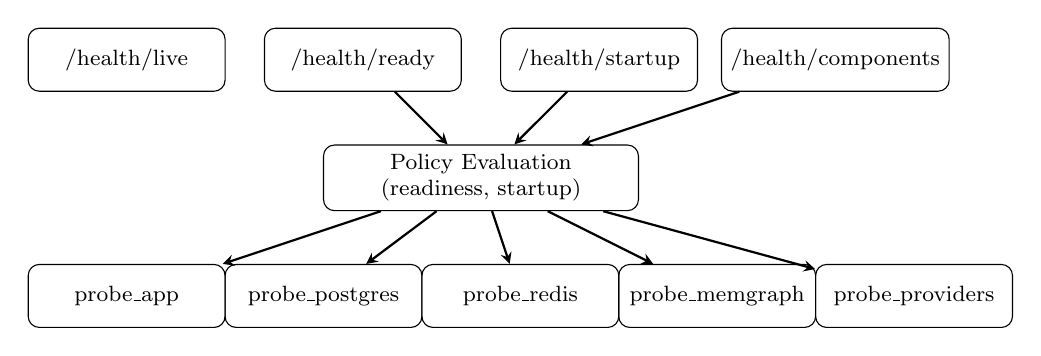
\begin{tikzpicture}[
    block/.style={draw, rounded corners, minimum width=2.5cm, minimum height=0.8cm, font=\footnotesize, align=center},
    arrow/.style={->, >=stealth, thick}
]
% Endpoints layer
\node[block] (live) at (0, 0) {/health/live};
\node[block] (ready) at (3, 0) {/health/ready};
\node[block] (startup) at (6, 0) {/health/startup};
\node[block] (comps) at (9, 0) {/health/components};

% Policy layer
\node[block, minimum width=4cm] (policy) at (4.5, -1.5) {Policy Evaluation\\(readiness, startup)};

% Component probes
\node[block] (app) at (0, -3) {probe\_app};
\node[block] (pg) at (2.5, -3) {probe\_postgres};
\node[block] (redis) at (5, -3) {probe\_redis};
\node[block] (mg) at (7.5, -3) {probe\_memgraph};
\node[block] (prov) at (10, -3) {probe\_providers};

% Arrows
\draw[arrow] (ready) -- (policy);
\draw[arrow] (startup) -- (policy);
\draw[arrow] (comps) -- (policy);
\draw[arrow] (policy) -- (app);
\draw[arrow] (policy) -- (pg);
\draw[arrow] (policy) -- (redis);
\draw[arrow] (policy) -- (mg);
\draw[arrow] (policy) -- (prov);
\end{tikzpicture}
\caption{Health probe system architecture showing the layered design from HTTP endpoints to component probes.}
\label{fig:health-probe-arch}
\end{figure}

\subsection{Probe Types and Endpoints}

The platform exposes four primary health endpoints:

\subsubsection{Liveness Probe (\texttt{/health/live})}

The liveness probe answers the question: ``Is this process alive and able to handle requests?''

\begin{lstlisting}[language=Python, caption={Liveness probe implementation}]
@router.get("/live", response_class=PlainTextResponse)
async def health_live() -> Response:
    """
    Liveness probe: returns simple 'ok' text for low-cost probes.
    Performs no external I/O and should be fast and stable.
    Always returns HTTP 200 with plain text "ok" body.
    """
    return PlainTextResponse(
        content="ok", 
        status_code=200, 
        headers={"Cache-Control": "no-store"}
    )
\end{lstlisting}

Characteristics:
\begin{itemize}
    \item \textbf{No external I/O}: Returns immediately without database or network checks
    \item \textbf{Plain text response}: Minimal overhead for frequent polling
    \item \textbf{Always 200}: If the code runs, the process is alive
    \item \textbf{Failure action}: Container restart by orchestrator
\end{itemize}

\subsubsection{Readiness Probe (\texttt{/health/ready})}

The readiness probe answers the question: ``Can this instance accept and process user traffic?''

\begin{lstlisting}[language=Python, caption={Readiness probe implementation}]
@router.get("/ready")
async def ready() -> Response:
    """
    Readiness probe: checks external dependencies and reports 
    aggregate status.
    
    Returns:
    - 200 when status is "ok" or "degraded" (with policy)
    - 503 when status is "error" (critical dependencies failed)
    """
    checks = await get_all_checks()
    status_str, http_code = evaluate_readiness(checks)
    body = build_response_body(
        checks=checks,
        status=status_str,
        service_name="cineca-agentic-platform",
        version=getattr(settings, "APP_VERSION", "0.1.0"),
    )
    
    # Check admin readiness flag (for graceful draining)
    if not _is_ready:
        body["status"] = "not ready"
        body["reason"] = "admin-disabled"
        return JSONResponse(status_code=503, content=body)
    
    return JSONResponse(status_code=http_code, content=body)
\end{lstlisting}

Characteristics:
\begin{itemize}
    \item \textbf{Dependency checks}: Tests PostgreSQL, Redis, and optional Memgraph
    \item \textbf{Policy-based aggregation}: Configurable required vs. optional components
    \item \textbf{Admin override}: Operators can mark instances as not-ready for draining
    \item \textbf{Failure action}: Remove from load balancer rotation
\end{itemize}

\subsubsection{Startup Probe (\texttt{/health/startup})}

The startup probe answers the question: ``Has this instance completed initialization and is it safe to begin health checks?''

\begin{lstlisting}[language=Python, caption={Startup probe with extended diagnostics}]
@router.get("/startup")
async def startup() -> Response:
    """
    Startup endpoint with rich diagnostics.
    Stricter than /ready: enforces migration requirements and 
    validates rate limit configuration.
    """
    checks = await get_all_checks()
    status_str, http_code, extras = evaluate_startup(checks)
    
    body = build_response_body(
        checks=checks,
        status=status_str,
        service_name="cineca-agentic-platform",
        version=getattr(settings, "APP_VERSION", "0.1.0"),
        extras=extras,  # Includes environment, limits, migrations
    )
    
    return JSONResponse(status_code=http_code, content=body)
\end{lstlisting}

The startup probe includes additional validation:
\begin{itemize}
    \item \textbf{Migration enforcement}: Verifies database migrations are applied when \texttt{ENFORCE\_MIGRATIONS=1}
    \item \textbf{Rate limit validation}: Warns if \texttt{RATE\_LIMIT\_MODE} is not \texttt{prod} in production
    \item \textbf{Environment diagnostics}: Reports configuration for troubleshooting
\end{itemize}

\subsubsection{Component Health (\texttt{/health/components})}

The component health endpoint provides granular visibility into individual system dependencies:

\begin{lstlisting}[language=Python, caption={Component health endpoint}]
@router.get("/components")
async def get_all_components() -> Response:
    """
    Get health status of all system components.
    Always returns 200 with individual component statuses.
    """
    checks = await get_all_checks()
    status_str, _ = evaluate_readiness(checks)
    
    body = build_response_body(
        checks=checks,
        status=status_str,
        service_name="cineca-agentic-platform",
        version=getattr(settings, "APP_VERSION", "0.1.0"),
    )
    
    return JSONResponse(status_code=200, content=body)
\end{lstlisting}

A single-component variant (\texttt{/health/components/\{name\}}) allows targeted health checks for specific dependencies.

\subsection{Probe Implementation Details}
\label{subsec:probe-implementation}

Each component probe follows a consistent pattern with timeout handling, retry logic, and structured result reporting.

\subsubsection{Component Check Data Model}

\begin{lstlisting}[language=Python, caption={ComponentCheck dataclass}]
class ComponentStatus(str, Enum):
    OK = "ok"           # Healthy and functional
    DEGRADED = "degraded"  # Functional with warnings
    ERROR = "error"     # Not functional
    UNKNOWN = "unknown" # Not configured/unreachable

@dataclass
class ComponentCheck:
    """Result of a component health probe."""
    ok: bool
    status: ComponentStatus
    latency_ms: int | None = None
    details: dict[str, Any] = field(default_factory=dict)
    
    def to_dict(self) -> dict[str, Any]:
        result = {"ok": self.ok, "status": self.status.value}
        if self.latency_ms is not None:
            result["latency_ms"] = self.latency_ms
        if self.details:
            result["details"] = self.details
        return result
\end{lstlisting}

\subsubsection{PostgreSQL Probe}

The PostgreSQL probe tests database connectivity with retry logic and pool statistics:

\begin{lstlisting}[language=Python, caption={PostgreSQL health probe}]
async def probe_postgres() -> ComponentCheck:
    """
    Probe PostgreSQL database connectivity.
    Tests connection with SELECT 1 query and reports pool statistics.
    """
    config = get_health_config()
    timeout_ms = getattr(config, "postgres_timeout_ms", 
                         config.db_timeout_ms)
    max_attempts = max(1, getattr(config, "postgres_retries", 2))
    
    for attempt in range(1, max_attempts + 1):
        try:
            is_healthy, error_msg = await asyncio.wait_for(
                asyncio.to_thread(check_db_health),
                timeout=timeout_ms / 1000.0
            )
            
            if is_healthy:
                return ComponentCheck(
                    ok=True,
                    status=ComponentStatus.OK,
                    latency_ms=latency_ms,
                    details={"database": "postgresql", 
                            "attempts": attempt},
                )
        except asyncio.TimeoutError:
            last_error = f"timeout after {timeout_ms}ms"
        # ... retry logic ...
    
    return ComponentCheck(
        ok=False,
        status=ComponentStatus.ERROR,
        details={"error": last_error, "attempts": max_attempts},
    )
\end{lstlisting}

\subsubsection{Redis Probe}

The Redis probe tests connectivity and reports job queue depths:

\begin{lstlisting}[language=Python, caption={Redis health probe with queue statistics}]
async def probe_redis() -> ComponentCheck:
    """
    Probe Redis connectivity and queue health.
    Tests PING command and reports queue depths for all job types.
    """
    client = await get_async_redis()
    pong = await asyncio.wait_for(client.ping(), timeout=timeout_seconds)
    
    if not pong:
        return ComponentCheck(
            ok=False, 
            status=ComponentStatus.ERROR,
            details={"error": "PING returned falsy"}
        )
    
    # Collect queue depths
    queues = {}
    for job_type in allowed_types:
        queue_key = f"jobs:queue:{job_type}"
        length = await client.llen(queue_key)
        queues[job_type] = length
    
    return ComponentCheck(
        ok=True,
        status=ComponentStatus.OK,
        latency_ms=latency_ms,
        details={"queues": queues} if queues else {}
    )
\end{lstlisting}

\subsubsection{Memgraph Probe}

The Memgraph probe tests graph database connectivity. It is marked as informational-only to avoid failing readiness when the graph database is temporarily unavailable:

\begin{lstlisting}[language=Python, caption={Memgraph health probe (informational)}]
async def probe_memgraph() -> ComponentCheck:
    """
    Probe Memgraph service (informational only).
    Failures are reported but don't affect readiness.
    """
    mg = Memgraph(host="memgraph", port=7687)
    
    result = await asyncio.wait_for(
        asyncio.to_thread(lambda: list(
            mg.execute_and_fetch("RETURN 1 AS ok LIMIT 1")
        )),
        timeout=2.0  # Generous timeout for thread pool contention
    )
    
    if result and result[0].get("ok") == 1:
        return ComponentCheck(
            ok=True,
            status=ComponentStatus.OK,
            latency_ms=latency_ms,
            details={"host": "memgraph:7687"}
        )
    
    return ComponentCheck(
        ok=True,  # Informational only
        status=ComponentStatus.DEGRADED,
        details={"note": "informational-only"}
    )
\end{lstlisting}

\subsubsection{LLM Provider Probe}

The provider probe checks the health of registered LLM providers:

\begin{lstlisting}[language=Python, caption={LLM provider health probe}]
async def probe_providers() -> ComponentCheck:
    """
    Probe provider registry health.
    Checks PostgreSQL provider registry and reports provider stats.
    """
    providers = await asyncio.wait_for(
        asyncio.to_thread(pg_repo.list_providers, tenant_id=None),
        timeout=config.db_timeout_ms / 1000.0
    )
    
    # Aggregate statistics
    total = len(providers)
    healthy = unhealthy = 0
    provider_details = []
    
    for provider in providers:
        health = pg_repo.get_provider_health(provider.get("name"))
        provider_healthy = health and health.get("reachable")
        
        if provider_healthy:
            healthy += 1
        else:
            unhealthy += 1
        
        provider_details.append({
            "name": provider.get("name"),
            "type": provider.get("type"),
            "status": "healthy" if provider_healthy else "unhealthy",
            "model": provider.get("model") or "no default model loaded",
        })
    
    status = (ComponentStatus.OK if unhealthy == 0 
              else ComponentStatus.DEGRADED)
    
    return ComponentCheck(
        ok=True,
        status=status,
        details={
            "total": total,
            "healthy": healthy,
            "unhealthy": unhealthy,
            "providers": provider_details,
        },
    )
\end{lstlisting}

\subsection{Component Registry}

The \texttt{ComponentRegistry} class manages the collection of probe functions and provides methods for probing individual components or all components in parallel:

\begin{lstlisting}[language=Python, caption={Component registry implementation}]
class ComponentRegistry:
    """Registry of all system components with their probe functions."""
    
    def __init__(self):
        self._components = {
            "app": probe_app,
            "postgres": probe_postgres,
            "redis": probe_redis,
            "memgraph": probe_memgraph,
            "providers": probe_providers,
            "workers": probe_workers,
            "ollama": probe_ollama,
            "prometheus": probe_prometheus,
            "grafana": probe_grafana,
        }
    
    async def probe_all(self) -> dict[str, ComponentCheck]:
        """Probe all components in parallel."""
        tasks = {name: self.probe(name) for name in self._components}
        results = await asyncio.gather(*tasks.values(), 
                                       return_exceptions=True)
        # ... result processing ...
        return checks
\end{lstlisting}

\subsection{Readiness Policy Evaluation}

The policy layer aggregates component health into overall service status:

\begin{lstlisting}[language=Python, caption={Readiness policy evaluation}]
def evaluate_readiness(checks: dict[str, ComponentCheck]) -> tuple[str, int]:
    """
    Evaluate readiness based on component checks.
    
    Policy:
    - Required components (app, postgres, redis) must be ok/degraded
    - Optional components can be degraded without failing readiness
    - Informational components don't affect readiness
    """
    config = get_health_config()
    required_ok = True
    has_degraded = False
    
    for name, check in checks.items():
        is_required = name in config.required_components
        
        if is_required:
            if check.status == ComponentStatus.ERROR:
                required_ok = False
            elif check.status == ComponentStatus.DEGRADED:
                has_degraded = True
        elif check.status in (ComponentStatus.DEGRADED, 
                              ComponentStatus.ERROR):
            has_degraded = True
    
    if not required_ok:
        return ("error", 503)
    elif has_degraded and not config.allow_degraded:
        return ("error", 503)
    elif has_degraded:
        return ("degraded", 200)
    else:
        return ("ok", 200)
\end{lstlisting}

\subsection{Kubernetes Integration}

The health endpoints are designed for direct use in Kubernetes pod specifications:

\begin{lstlisting}[language=yaml, caption={Kubernetes probe configuration example}]
livenessProbe:
  httpGet:
    path: /health/live
    port: 8000
  initialDelaySeconds: 5
  periodSeconds: 10
  timeoutSeconds: 3
  failureThreshold: 3

readinessProbe:
  httpGet:
    path: /health/ready
    port: 8000
  initialDelaySeconds: 10
  periodSeconds: 15
  timeoutSeconds: 10
  failureThreshold: 2

startupProbe:
  httpGet:
    path: /health/startup
    port: 8000
  initialDelaySeconds: 0
  periodSeconds: 5
  timeoutSeconds: 30
  failureThreshold: 30  # 2.5 minutes max startup time
\end{lstlisting}

\subsection{Admin Readiness Control}

Operators can manually toggle instance readiness for graceful deployment draining:

\begin{lstlisting}[language=Python, caption={Admin readiness toggle endpoint}]
@router.post("/startup/readiness", include_in_schema=False)
async def set_startup_readiness(state: str, request: Request, 
                                 auth=Depends(_require_admin)) -> Response:
    """
    Set readiness state for this instance.
    Accepts 'ready' or 'not-ready'.
    Used for rolling updates to drain traffic before shutdown.
    """
    if state.lower() == "ready":
        set_ready(True)
        return JSONResponse(status_code=200, content={"status": "ready"})
    
    if state.lower() in {"not-ready", "not_ready", "notready"}:
        set_ready(False)
        return JSONResponse(status_code=200, 
                           content={"status": "not ready"})
    
    raise HTTPException(status_code=400, 
                       detail="invalid state; use 'ready' or 'not-ready'")
\end{lstlisting}

This endpoint requires admin authentication (either \texttt{X-Admin-Token} header or JWT with admin scope) and logs state changes for audit purposes.

